\documentclass[twocolumn]{report}
\usepackage{amsfonts}
\usepackage{amsmath}
\usepackage{tikz}
\usepackage{pgfplots}
\usepackage{ngerman}
\usepackage[hidelinks]{hyperref}

\pgfplotsset{width=7cm,compat=1.18}

\title{\textbf{Das Diffie-Hellman Verfahren}}
\author{Tim Teichmann}
\date{\today}

\begin{document}
\maketitle

\section*{Funktionsweise}
Alice und Bob möchten sicher miteinander kommunizieren.
Das funktioniert indem sie einen gemeinsamen Schlüssel bestimmen,
mit dem sie ihre Nachrichten verschlüsseln können. Dieser gemeinsame
Schlüssel sollte nur den beiden bekannt sein.

Um sicher einen gemeinsamen Schlüssel zu bestimmen, können Alice und Bob
zwei Zahlen $p\in\mathbb{P},g\in\mathbb{N},g<p$ wählen.

Alice und Bob wählen außerdem jeweils einen privaten Schlüssel $a,b\in\mathbb{N}$.
Außerdem berechnen beiden einen öffentlichen Schlüssel $A,B$, den sie miteinander teilen.
\begin{align}
    A=g^a \mod p \\
    B=g^b \mod p
\end{align}
Nun bestimmen beide jeweils einen gemeinsamen Schlüssel $K_1$ und $K_2$.
\begin{align}
    K_1=B^a \mod p \\
    K_2=A^b \mod p
\end{align}
Sind die Parameter richtig gewählt, so gilt $K_1=K_2$:
\begin{align}
    K_1&=B^a \mod p \\
    &=\left(g^b \mod p\right)^a \mod p \\
    &=g^{ba} \mod p \\
    K_2&=A^b \mod p \\
    &=\left(g^a \mod p\right)^b \mod p \\
    &=g^{ab} \mod p \\
    &=g^{ba} \mod p \\
    &=K_1
\end{align}
Alice kann Bob Nachrichten schicken, die mit dem Schlüssel $K_1$ verschlüsselt wurden.
Bob kann diese mit seinem Schlüssel $K_2$ entschlüsseln.

\section*{Sicherheit}
Eine dritte (Celine) kann die Kommunikation zwischen Alice und Bob abfangen.
Celine sind also die Werte von $p,g,A$ und $B$ bekannt.

Um den Wert von einer der geheimen Variablen $a$ oder $b$ zu bestimmen,
muss Celine eine der folgenden Gleichungen lösen:
\begin{align}
    A=g^a \mod p \\
    B=g^b \mod p
\end{align}
In diesem Beispiel gehen wir davon aus, dass $p=13,g=2,A=8$ und $B=4$ ist.
Die geheimen Werte sind $a=3,b=2$ und $K=12$, diese kennt Celine jedoch nicht.

Celine wählt in diesem Beispiel die erste Gleichung.
Sie bemerkt schnell, dass es sehr viel leichter wäre den
Wert von $a$ zu bestimmen, wenn der öffentliche Schlüssel durch
die Gleichung $A=g^a$ berechnet würde.
In diesem Fall könnte man nämlich eine Umkehroperation der Exponentiation,
den Logarithmus, verwenden:
\begin{align}
    A&=g^a \\
    \Leftrightarrow \ln{A}&=\ln{g^a} \\
    \Leftrightarrow \ln{A}&=a\ln{g} \\
    \Leftrightarrow \frac{\ln{A}}{\ln{g}}&=a \\
    \Leftrightarrow a&=\frac{\ln{A}}{\ln{g}}
\end{align}
Die Berechnung von $A=g^a\mod p$ ist die diskrete Exponentiation.
Die Umkehroperation ist der diskrete Logarithmus.

Während man den normalen Logarithmus effizient berechnen kann, existiert
bis heute kein Algorithmus mit dem man den diskreten Logarithmus effizient
berechnen kann.

Der Modulo ist dafür verantwortlich, dass dieses Problem des diskreten
Logarithmus nicht effizient gelöst werden kann.
Im Gegensatz zu $g^a$ (in unserem Fall $2^a$) wiederholen sich die Werte
der Gleichung mit Modulo immer wieder:

\begin{center}
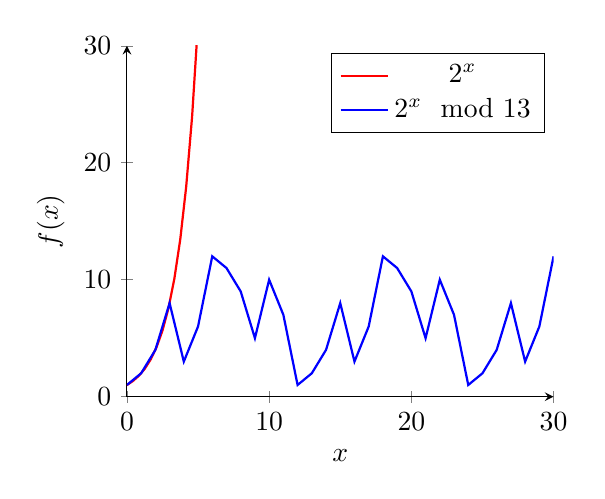
\begin{tikzpicture}
\begin{axis}[xmin=0,
             xmax=30,
             ymin=0,
             ymax=30,
             axis lines=left,
             xlabel=$x$,
             ylabel=$f(x)$]
    \addplot [samples=25,color=red,thick] {2^x};
    \addlegendentry{$2^x$}

    \addplot [color=blue,thick] coordinates {
        (0,1) (1,2) (2,4)
        (3,8) (4,3) (5,6)
        (6,12) (7,11) (8,9)
        (9,5) (10,10) (11,7)
        (12,1) (13,2) (14,4)
        (15,8) (16,3) (17,6)
        (18,12) (19,11) (20,9)
        (21,5) (22,10) (23,7)
        (24,1) (25,2) (26,4)
        (27,8) (28,3) (29,6)
        (30,12)
    };
    \addlegendentry{$2^x\mod 13$}
\end{axis}
\end{tikzpicture}
\end{center}
Celines Ziel ist also einen Schnittpunkt zwischen
den Funktionen $f(x)=8$ (da $A=8$)
und $g(x)=2^x\mod 13$ (da $g=2$ und $p=13$) zu finden.

Die Funktion $h(x)=2^x$ hat nur einen Schnittpunkt mit $f(x)$.

Wie man relativ gut an der folgenden Grafik erkennen kann,
gibt es unendlich viele Schnittpunkte zwischen diesen beiden
Funktionen. Es existieren also unendlich viele geheime Schlüssel $a$,
die zum richtigen gemeinsamen Schlüssel $K=12$ führen.

\begin{center}
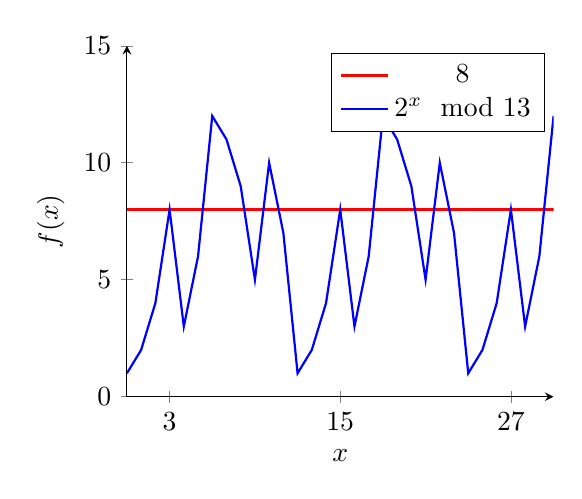
\begin{tikzpicture}
\begin{axis}[xmin=0,
             xmax=30,
             ymin=0,
             ymax=15,
             axis lines=left,
             xlabel=$x$,
             ylabel=$f(x)$,
             xtick={3,15,27}]
    \addplot [domain=0:30,samples=2,color=red,thick] {8};
    \addlegendentry{$8$}

    \addplot [color=blue,thick] coordinates {
        (0,1) (1,2) (2,4)
        (3,8) (4,3) (5,6)
        (6,12) (7,11) (8,9)
        (9,5) (10,10) (11,7)
        (12,1) (13,2) (14,4)
        (15,8) (16,3) (17,6)
        (18,12) (19,11) (20,9)
        (21,5) (22,10) (23,7)
        (24,1) (25,2) (26,4)
        (27,8) (28,3) (29,6)
        (30,12)
    };
    \addlegendentry{$2^x\mod 13$}
\end{axis}
\end{tikzpicture}
\end{center}
Grundsätzlich sind nur ganze Schlüssel relevant.
Anhand von der Grafik lässt sich erkennen, dass
$a_1=3,a_2=15$ und $a_3=27$ ganze Schlüssel sind,
die zum richtigen Ergebnis führen.

Für $p=13,g=2$ und $A=8$ sind also alle
\begin{align}
    a=3+12n,\quad n\in\mathbb{N}_0  
\end{align}
geheime Schlüssel von Alice.

Bevor sich $g(x)$ das erste mal wiederholt, müssten alle ganzen Zahlen
ausprobiert werden, für die $h(x)\leq p$ ist.

In echten Anwendungen ist $p$ normalerweise mindestens
2048-bit lang.
Eine 2048-Bit lange Primzahl $p$ hat in etwa 617 Dezimalstellen, da
ein Bit die Werte 0 oder 1 annehmen kann, während eine Dezimalzahl
einen Wert zwischen 0 und 9 annehmen kann:
\begin{align}
    2^{2048}&=10^n \\
    \Leftrightarrow \ln{2^{2048}}&=\ln{10^n} \\
    \Leftrightarrow 2048\ln{2}&=n\ln{10} \\
    \Leftrightarrow \frac{2048\ln{2}}{\ln{10}}&=n \\
    \Leftrightarrow n &\approx 616.51 \approx 617
\end{align}
Die kleinste ganze Zahl mit 617 Dezimalstellen ist $10^{616}$.
Diese Zahl ist bei weitem zu groß um in die Integer-Datentypen
gängiger Programmiersprachen zu passen.
Der größte Integer-Datentyp der Programmiersprache C (\textit{unsigned long long} bzw.
\textit{unsigned long long int}) ist beispielsweise
mindestens 64-Bit groß.
\footnote{Quelle: \url{https://en.wikipedia.org/wiki/C_data_types},\\
Abrufdatum: 11.01.24}

Die Rede ist von mindestens 64-Bit,
da die echte größe der Datentypen stark abhängig von der
Platform ist, für die ein C Programm kompiliert wird.
Da viele C-Kompiler existieren gibt es einen offenen C-Standard,
der -- unter anderem -- diese Mindestgrößen definiert.

Die größen für die Datentypen \textit{unsigned long long} und
\textit{unsigned long long int} wurden im Standard C99 definiert.
\footnote{Quelle: \url{https://en.wikipedia.org/wiki/C99},\\
Abrufdatum: 11.01.24}
\end{document}
